\documentclass{article}

\usepackage{graphicx}
\usepackage{tikz}
\usepackage{tikzsymbols}
\usetikzlibrary{calc,patterns,shapes.geometric}
\pagestyle{empty}
\usepackage[margin=0pt]{geometry}
\geometry{papersize={14in,12in}}

\def\centerarc[#1](#2)(#3:#4:#5){\draw[#1] ($(#2)+({#5*cos(#3)},{#5*sin(#3)})$) arc (#3:#4:#5);}

\begin{document}
	\begin{figure}
		\centering
		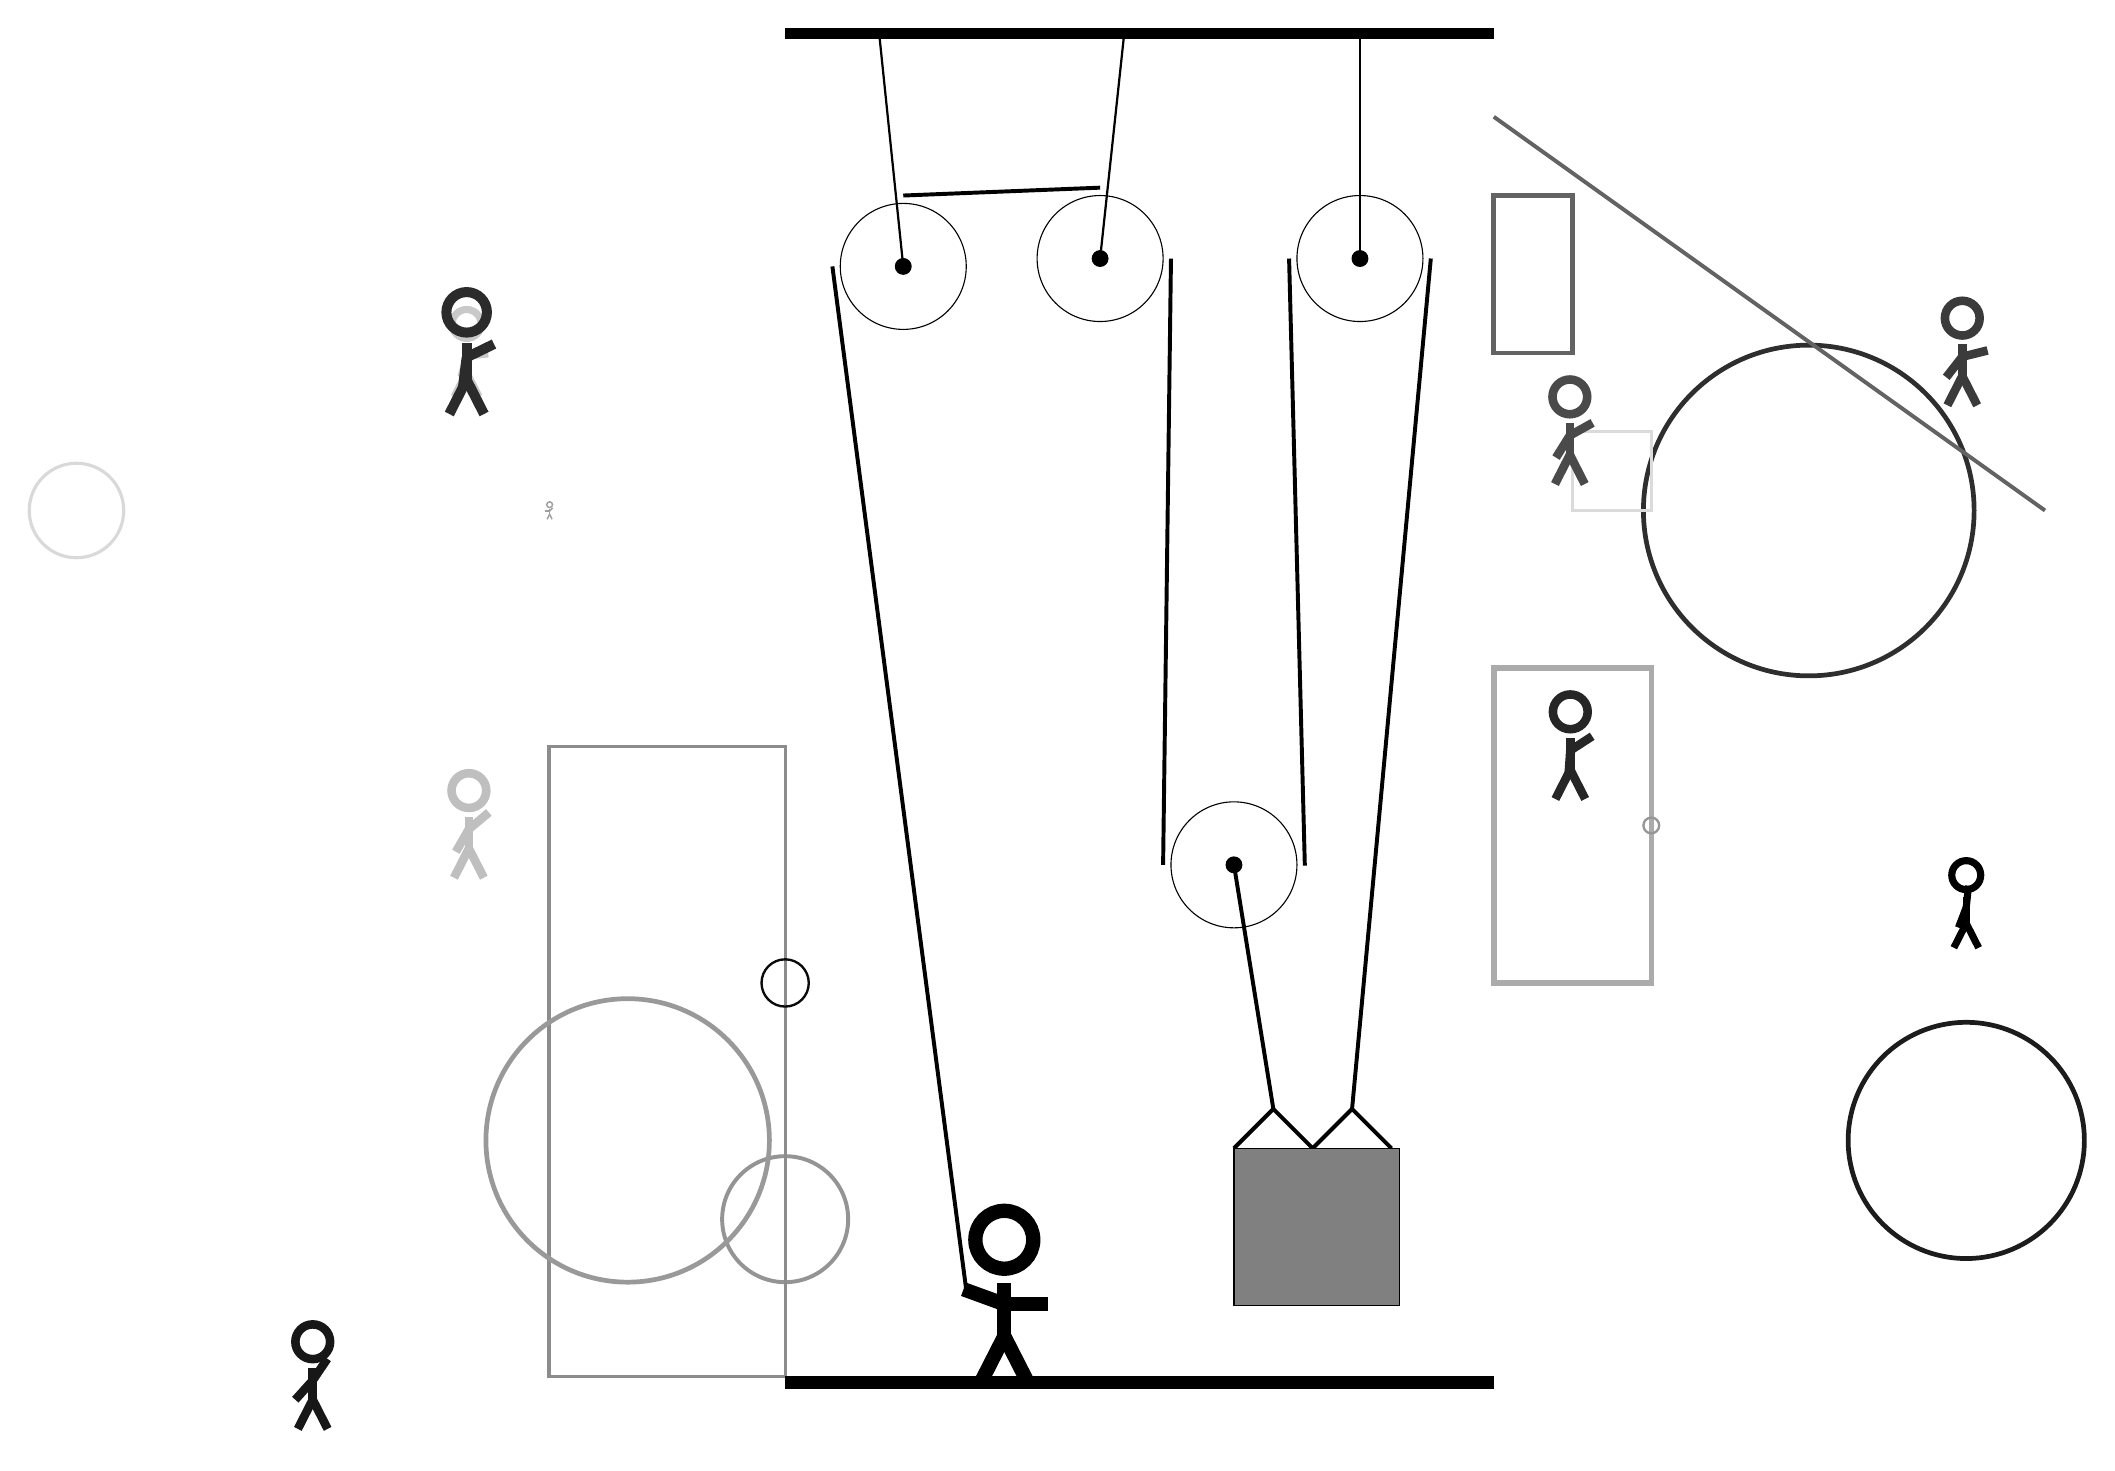
\begin{tikzpicture}
			%%%%% START %%%%%
			
			\draw[fill=black] (-3, 14) rectangle (6, 14.125);
			
			\draw (1, 11.2) circle (0.8);
			\draw[fill=black] (1, 11.2) circle (0.1);
			\draw[thick] (1, 11.2) -- (1.3, 14);
			
			\draw (4.3, 11.2) circle (0.8);
			\draw[fill=black] (4.3, 11.2) circle (0.1);
			\draw[thick] (4.3, 11.2) -- (4.3, 14);
			
			\draw [line width=0.5mm, color=black!42](-3, -1) circle (0.8);
			
			\draw [line width=0.4mm, color=black!15](-12, 8) circle (0.6);
			\draw [line width=0.6mm, color=black!82](10, 8) circle (2.1);
			\draw [line width=0.6mm, color=black!89](12, 0) circle (1.5);
			\node[line width=0.6mm, color=black!25] at (-7, 4) {\Strichmaxerl[6][60][40]};
			\node[line width=0.6mm, color=black!21] at (-7, 10) {\Strichmaxerl[5][75][6]};
			\node[line width=0.3mm, color=black!38] at (-6, 8) {\Strichmaxerl[1][0][47]};
			
			\node[line width=0.3mm, color=black!83] at (-7, 10) {\Strichmaxerl[7][83][26]};
			\draw[line width=0.7mm, color=black!33] (6, 2) rectangle (8, 6);
			
			\node[line width=0.7mm, color=black!85] at (7, 5) {\Strichmaxerl[6][86][33]};
			\draw[line width=0.4mm, color=black!45] (-3, 5) rectangle (-6, -3);
			
			\draw[line width=0.2mm, color=black!67] (-3, 2) rectangle (-3, 2);
			\node[line width=0.3mm, color=black!100] at (12, 3) {\Strichmaxerl[5][69][84]};
			\draw[line width=0.6mm, color=black!61] (7, 10) rectangle (6, 12);
			\draw[line width=0.5mm, color=black!61](6, 13) -- (13, 8);
			\draw [line width=0.6mm, color=black!40](-5, 0) circle (1.8);
			\draw[line width=0.4mm, color=black!14] (7, 9) rectangle (8, 8);
			
			\draw [line width=0.3mm, color=black!41](8, 4) circle (0.1);
			\node[line width=0.6mm, color=black!71] at (7, 9) {\Strichmaxerl[6][58][29]};
			\draw [line width=0.3mm, color=black!96](-3, 2) circle (0.3);
			\node[line width=0.6mm, color=black!91] at (-9, -3) {\Strichmaxerl[6][48][56]};
			\node[line width=0.6mm, color=black!77] at (12, 10) {\Strichmaxerl[6][52][14]};
			
			
			\draw (2.7, 3.5) circle (0.8);
			\draw[fill=black] (2.7, 3.5) circle (0.1);
			
			\draw[line width=0.5mm]  (2.7, -0.1) -- (3.2, 0.4) -- (3.7, -0.1) -- (4.2, 0.4) -- (4.7, -0.1);
			\draw[fill=black!50] (2.7, -0.1) rectangle (4.8, -2.1);
			
			\draw (-1.5, 11.1) circle (0.8);
			\draw[fill=black] (-1.5, 11.1) circle (0.1);
			\draw[thick] (-1.5, 11.1) -- (-1.8, 14);
			
			\draw[line width=0.5mm](-0.7, -1.9) --  (-2.4, 11.1);
			\centerarc[line width=0.5mm](-1.5, 11.1)(90:180:0.9);
			\draw[line width=0.5mm](-1.5, 12.0) -- (1, 12.1);
			\centerarc[line width=0.5mm](1, 11.2)(0:90:0.9);
			\draw[line width=0.5mm](1.9, 11.2) -- (1.8, 3.5);
			\centerarc[line width=0.5mm](2.7, 3.5)(180:370:0.9);
			\draw[line width=0.5mm] (3.6, 3.49) -- (3.4, 11.2);
			\centerarc[line width=0.5mm](4.3, 11.2)(0:180:0.9);
			\draw[line width=0.5mm](4.2, 0.4) -- (5.2, 11.2);
			\draw[line width=0.5mm] (3.2, 0.4) -- (2.7, 3.5);
			
			\node at (-0.2, -2) {\Strichmaxerl[10][-20][0]};
			
			\draw[fill=black] (-3, -3) rectangle (6, -3.15);
			
			%%%%% END %%%%%
		\end{tikzpicture}
	\end{figure}	
\end{document}